\chapter{Unit Tests}

Im vorliegenden Projekt wurden Unit Tests eingesetzt, um die Qualität der Software zu sichern und Fehler frühzeitig zu erkennen. Die implementierten Tests konzentrieren sich hauptsächlich auf die \href{https://github.com/MichaelaHaag/RezeptApp/blob/main/3-Domain-Code/src/test/java/de/rezeptapp/domain/Rezept}{\code{Domain Code Schicht}} und \href{https://github.com/MichaelaHaag/RezeptApp/tree/main/1-Adapter/src/test/java/de/rezeptapp/adapter/Datenpersistenz}{\code{Adapters-Schicht}}, da hier die Funktionalität des Codes von größter Bedeutung ist. Hier wurden allerdings nur exemplarische Klassen getestet. Für die Peripherie der Software in der Plugin-Schicht wurde zunächst auf Unit Tests verzichtet, da dieser Teil des Programms ohnehin leicht und häufig austauschbar sein soll und daher von geringerer Wichtigkeit ist, sodass ihm auch beim Testen eine geringere Priorität zugewiesen wurde.                              

Um eine möglichst korrekte Implementierung der Software zu erreichen, wird die AAA-Normalform angewendet. Die AAA-Normalform strukturiert jeden Unit Test in drei Bereiche: Arrange (Initialisierung der Testumgebung), Act (Ausführung der zu testenden Aktion) und Assert (Überprüfung der Testergebnisse).

\section{ATRIP-Regeln}

Die ATRIP-Regeln sind fünf grundlegende Regeln für Unit Test, welche verwendet werden, um sicherzustellen, dass die Tests klar, verständlich und effektiv sind. So steht jeder Buchstabe für eine Regel. In den nachfolgenden Abschnitten wird untersucht, wie sie in diesem Projekt angewendet wurden.

\subsection{Automatic}
Das A steht für Automatic und besagt, dass alle Test eigenständig ablaufen müssen und keine manuellen Eingriffe notwendig sein sollten. Die Tests müssen ihre Ergebnisse selbst überprüfen und anschließen bestanden oder nicht bestanden zurückgeben. In der Rezept-Anwendung laufen alle implementierten Unit Tests vollständig eigenständig ab, da keinerlei manuelle Eingriffe, etwa in Form von Werteeingaben, notwendig sind. Außerdem überprüfen alle Tests ihre Ergebnisse durch Assertions automatisch, dass diese den im Code eingetragenen erwarteten Ergebnissen entsprechen. Die Tests werden durch JUnit 5 automatisch ausgeführt. Nach dem Durchlaufen eines Testes wird das Testergebnis in \enquote{bestanden} oder \enquote{nicht bestanden} klassifiziert. IntelliJ bestätigt ein erfolgreiches Durchlaufen aller Tests mittels eines grünen Hakens.

\subsection{Thorough}
Die zweite Regel Thorough besagt, dass gute Tests alles Notwenige testen. Es soll jede missionskritische Funktionalität getestet werden. Allerdings ist eine eindeutige Entscheidung, ob alles Notwendige getestet wurde und damit die Regel erfüllt ist, schwierig. Als „notwendig“ wurde für das vorliegende Projekt die wesentliche Businesslogik und damit die Adapters-Schicht definiert. Diese wird mit einer hohen Testabdeckung (Code Coverage) getestet, sodass die implementierten Tests durchaus als gründlich bezeichnet werden können (vgl. \autoref{CodeCoverage}). Da ohne den Domain-Code nichts funktionieren würde und dieser langfristig kaum verändert werden soll, wurden hier auch exemplarische Methoden getestet. Da die Software zum Zeitpunkt der Verfassung noch nicht von Endanwendern ausgiebig getestet worden war und bis dahin keine Softwarefehler gemeldet wurden, wurden keine spezifischen Tests für Softwarefehler implementiert.

\subsection{Repeatable}
Das R in den ATRIP-Regeln bedeutet Repeatable und besagt, dass, jeder Unit Test automatisch durchführbar sein sollte und kontinuierlich das gleiche Testergebnis liefern sollte, da sie weder zeit- noch zufallsabhängige Komponenten beinhalten und keine Abhängigkeiten auf Datenbanken oder Dateisystemen haben. Um zuverlässige Tests für die variablen Komponenten zu gewährleisten, wird auf Mock-Objekte zurückgegriffen, da sie kontinuierlich konsistente Daten an den Test liefern. (siehe \autoref{Mocks})


\subsection{Independent}
Das I steht für Independent und besagt, dass die Unit Tests jederzeit in beliebiger Reihenfolge ausführbar sein müssen. Dies wird sichergestellt, indem die Unit Tests keine impliziten Abhängigkeiten untereinander besitzen und die AAA-Normalform strikt befolgt wird, also jeder Test in seiner ersten Phase seine eigene „Testwelt“ initialisiert. Im Produktivbetrieb gibt es Abhängigkeiten auf persistierte Daten. Um dieses in den Unit Tests zu verhindern, werden jegliche Persistenzzugriffe auf Mocks ausgeführt, welche in der ersten Phase jedes Tests neu trainiert werden.

\subsection{Professional}
Die letzte Regel, Professional, besagt, dass die Unit Tests eine einheitliche, leicht verständliche Syntax und übersichtliche Struktur vorweisen  sollen, um den Umgang und das Weiterentwickeln im professionellen Bereich zu vereinfachen. Durch gleiche Namenskonventionen, die aus der Ubiquitous Language hervorgehen, und der Aufbau der Tests nach der AAA-Normalform wird das Kriterium an diese Regel erfüllt. Zu dem professionellen Standard gehört zudem, dass die Dateinamen und die Programmcodes der Tests verständlich und nachvollziehbar sind. Hierfür hat die Testklasse denselben Namen wie die zu testende Klasse nur mit dem Suffix \enquote{Test}. Bei den Testmethoden gilt dasselbe, nur mit dem Präfix \enquote{test\_}. Dadurch soll die Zuordnung der Methoden zu den jeweiligen Unit Tests vereinfacht werden. 


\section{Code Coverage}
\label{CodeCoverage}

Code Coverage ist eine Metrik, die verwendet wird, um den Umfang zu messen, in dem ein Softwareprogramm während der Testausführung getestet wird. Es misst den Prozentsatz der Codezeilen, die im Rahmen des Testverfahrens erfolgreich durchlaufen wurden.
In der Softwareentwicklung wird häufig Gebrauch von der Line Coverage und der Branch Coverage gemacht. Die Line Coverage gibt den Anteil der durchlaufenen Codezeilen von allen möglichen Codezeilen mit ausführbaren Befehlen an. Die Branch Coverage gibt den Anteil der durchlaufenen Abzweigungen (if-Konditionen oder Schleifen) von allen möglichen Abzweigungen an.

\autoref{fig:CodeCoverageBild} zeigt eine Messung der Code Coverage der IDE IntelliJ IDEA für die Anwendung. So beträgt die Line Coverage insgesamt 33\% und die aussagekräftigere Branch Coverage (in der Abbildung, die Spalte \enquote{Block}) sogar 44,8\%. Insgesamt wird bei der Code Coverage solch ein niedriges Ergebnis erreicht, da nur eine geringe Anzahl an exemplarischen Tests erstellt wurde. 
In der Adapters-Schicht ist die Branch Coverage hoch, jedoch ist die Line Coverage niedrig, da vergleichsweise nur sehr wenige Codezeilen getestet wurden. In der Domain-Schicht ist es genau umgekehrt. Hier ist die Line Coverage mit 64\% sehr hoch, da sehr viele Methoden ausführlich getestet wurden, jedoch ist die Branch Coverage deutlich niedriger, da hier weniger Abzweigungen getestet wurden. 

Besonders gut ist dabei das Einhalten der Dependency Rule zu sehen: Da nur die Adapters-Schicht und das Rezept Package des Domain Codes getestet wurden, hat die Plugin-Schicht keinerlei Testabdeckung. Der Domain Code \code{Kategorie}, welcher keine eigenen Tests besitzt, ist zu unserem Überraschen hingegen zu großen Teilen getestet. Dies lässt sich durch eine bestehende Abhängigkeit von der getesteten Adapters-Schicht erklären.

\begin{figure}[ht]
	\centering
	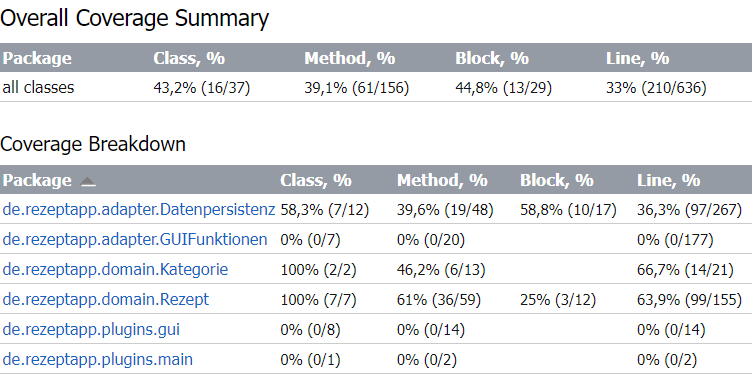
\includegraphics[width=0.90\textwidth]{Bilder/CodeCoverage.png} 
	\caption{Code Coverage der Rezept-App}
	\label{fig:CodeCoverageBild}
\end{figure}

\section{Mock-Objekte}
\label{Mocks}

Mock-Objekte (Mocks) werden stellvertretend für reale Softwareobjekte verwendet, um eine Klasse isoliert zu testen. Wie in der Repeatable ATRIP-Regel bereits benannt, ersetzten Mock-Objekte die Abhängigkeiten von Klassen als Objekt mit der für den Unit Test benötigten Funktionalität. Im Rahmen dieses Softwareprojektes wurde auf das Mocking-Framework EasyMock und Testing-Framework JUnit 5 zurückgegriffen.

Verwendet werden die Mock-Objekte in der \href{https://github.com/MichaelaHaag/RezeptApp/blob/main/3-Domain-Code/src/test/java/de/rezeptapp/domain/Rezept/RezeptRepositoryTest.java}{\code{RezeptRepositoryTest}} Klasse. Da hier eine Dependency Inversion durchgeführt wurde, erhalten alle Methoden als Eingabeparameter ein \code{IEntityManger}-Objekt. Dieses wird für die Unit Tests durch Mocks ersetzt, welche die für den jeweiligen Test notwendigen Daten liefern. Ein Beispiel für eine Testmethode, welche ein Mock verwendet, ist \code{test\_findeZutat()}, in welchem der \code{EntityManager} gemockt wird. Dazu wird das Mock-Objekt zunächst durch EasyMock erstellt, anschließend trainiert und aktiviert. Im Training wird dem Mock-Objekt beigebracht, auf den Methodenaufruf \code{finde()} ein bestimmtes Zutat-Objekt zurückzugeben. Abschließend wird überprüft, ob das zurückgegebene Objekt mit dem erwarteten Objekt übereinstimmt und ob das Mock-Objekt richtig verwendet wurde. 
